% Files using this must be two subfolders
% deep. Adjust the number of ../ for the
% depth of the file.
% Imports
\usepackage{fancyhdr}
\usepackage{geometry}
\usepackage{icomma}
\usepackage{amsmath}
\usepackage{multicol}
\usepackage{mathptmx}
\usepackage{anyfontsize}
\usepackage{t1enc}
\usepackage{tabto}
\usepackage{listings}
\usepackage{filecontents}
\usepackage{subcaption}
\usepackage{tikz}
\usepackage[parfill]{parskip}
\usepackage{graphicx}
\usepackage[]{mdframed}
\usepackage{amsmath}
\usepackage[makeroom]{cancel}
\usepackage{pgfplots}
\usepackage{pgfplotstable}
\usepackage{xfrac}
\usepackage{amssymb}
\usepackage{mathtools}
\pgfplotsset{compat=1.18}
\usetikzlibrary{patterns}
\usepgfplotslibrary{polar}
\usepgfplotslibrary{fillbetween}

\geometry{margin=2.5cm}

\newcommand{\name}{Kaleb Burris}
\newcommand{\classname}{MATH F253, Elizabeth S. Allman, University of Alaska Fairbanks}
\newcommand{\assignment}{FILL IN ASSIGNMENT NAME}

\pagestyle{fancy}

\fancyhead[L]{
    \name 
    \newline
    \classname
    \newline
    \assignment
}

\newcommand{\horizontal}{\noindent\rule{\hsize}{0.4pt}}

\setlength{\headheight}{42pt}
\setlength{\headsep}{0.25in}
\setlength{\columnsep}{0.35cm}
\setlength{\columnseprule}{1pt}

\usepackage[T1]{fontenc}
\usepackage{lmodern}

\usepackage{graphicx}
\usepackage[]{mdframed}

\graphicspath{ {./images/} }

% Put class number, class name, and professor 
% name.
\renewcommand\classname{STAT F300 Statistics, Dr. Short}

% Put the assignment name with \S if 
% necessary for the section and the question 
% numbers.
\renewcommand\assignment{Homework 2, Due Friday, January 27, 23:59}

\begin{document}

    % Templates
    \iffalse
    % Use these for equations.
    \begin{equation*}
        \begin{gathered}
            Equations go here.
        \end{gathered}
    \end{equation*}

    % Use this if a line of math is too long.
    \resizebox{\hsize}{!}{$Long equation goes here$}

    % Use these for multiple columns.
    \begin{multicol*}{# of columns}
        % Remove the * if you want the columns to be balanced.
    \end{multicol*}

    % Use this to add a horizontal line.
    \horizontal

    \fi

    % Begin homework here.
    %%%%%%%%%%%%%%%%%%%%%%

    \paragraph*{1.}
    \begin{mdframed}
        Done.
    \end{mdframed}

    \paragraph*{2.}
    Use R to construct a stem-and-leaf plot of this data set:

    \{66, 66, 69, 74, 74, 75, 75, 76, 76, 76, 76, 78, 79, 79, 81, 81, 82, 83, 83, 84, 86, 87, 87, 92, 98\}

    \begin{mdframed}
        \begin{lstlisting}[language=R]
> x <- c(66, 66, 69, 74, 74, 75, 75, 76, 76, 76, 76, 
78, 79, 79, 81, 81, 82, 83, 83, 84, 86, 87, 87, 92, 98)
> x <- sort(x)
> stem(x)

    The decimal point is 1 digit(s) to the right of the |

    6 | 669
    7 | 44556666899
    8 | 112334677
    9 | 28
        \end{lstlisting}
    \end{mdframed}

    Also, what is a fairly typical value, based on the stem-and-leaf plot?

    \begin{mdframed}
        It looks like 7 is a typical value, followed closely by 8.
    \end{mdframed}

    \paragraph*{3}
    Construct a dot plot of this data set: \{2,3,3,0,12, 0,1,4,6,2, 0,6,5,9,8, 1,1,1,2,3, 10,4,5,5,1\}

    \begin{mdframed}
        \begin{multicols*}{2}
        \begin{lstlisting}[language=R]
> x <- c(2,3,3,0,12, 0,1,4,6,2, 
0,6,5,9,8,1,1,1,2,3,10,4,5,5,1)
> stripchart(x, method="stack", 
offset=0.5, at=0.15, pch=20)
        \end{lstlisting}

        \resizebox{}{\textwidth}{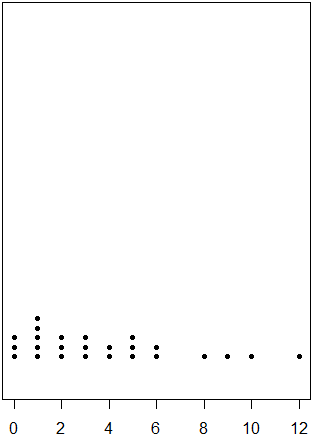
\includegraphics{Rplot_1}}
    \end{multicols*}
    \end{mdframed}

\end{document}